% !TeX root = ../../Thesis.tex
\chapter{Theory}
\label{chp:theory}

Remember to refer to Notes for Cours Ecole Doctorale, Advanced Theory of Plasmas, Ecole Polytechnique Fédérale de Lausanne (Saved on Mendeley)

\section{Motivation}
\subsection{Kinetic plasma instabilities}
\subsection{Three-wave parametric instabilities}

\section{Linear theory}
The aim of the linear theory of \acrshort{SBS} is to understand how the growth
 of the instability depends on factors such as: plasma density; laser intensity; and temperature.
\subsection{Dispersion curves and linear modes}
\subsection{Zoology/topology of modes}
\subsubsection{Beam acoustic modes}
\subsubsection{Electron acoustic modes}
ie on the omega,k diagram how many things are there that we should be worried
about? BGK modes, B\cite{Kruer96}
\subsection{Landau damping}

\section{Quasi-linear theory}
%\subsection{Landau damping}

A key aspect of quasilinear theory is its identification of the distinction between reso-
nant and non-resonant particles, scattering and diffusion \citep{Sagdeev2018}.

Bohm-Gross waves; Beam acoustic modes, other acoustic modes.
etc. Where are they and how do they relate? Ie the Bohm-Gross and Electron
Acoustic modes join at klD~0.53

\section{Nonlinear theory}
\subsection{Three-wave parametric instabilities}
\subsection{Nonlinear frequency shift}
\subsection{Nonlinear Landau damping}
%non-linear basis for trapping induced SRS modes found in \cite{Rose2001}, also
 %a thing called the nonlinear dielectric function

\subsection{Rosenbluth gain for SRS}

Since the instability we are concerned with is convective, we would like to understand what the maximum wave amplitude is for the daughter waves, according to the linear theory, in order to determine how SRS will grow in the fluid regime.

The derivation below follows the the steps laid out in \citet{Nishikawa1976}, with the following adapatations for this thesis:some steps written out in more explicit detail; notation changes, to improve the readability; and minor typographical corrections. 

We use our physical understanding of the system make the following assumptions:
\begin{enumerate}
	\item undamped EMW $\Gamma_1 = 0$
	\item strong damping and slow convection of EPW
	\item constant source at 0, maximum value at $+\infty$
	\item perfect matching at $x=0$, assume kappa is well-approximated by 
	$\kappa(x) = \kappa'(0)x$.
\end{enumerate}

Consider a three-wave parametric instability that takes place in a plasma slab with a density gradient in $x$ with a uniform pump. The density gradient leads to $x$-varying wavenumbers for the waves, so we define the `wavenumber mismatch' as $\kappa = k_0(x) - k_1(x) - k_2(x)$, where perfect matching is defined by the condition $\kappa(x=0) = 0$ and we insist that $\kappa = \kappa' x$. The daughter waves can be described by the following pair of partial differential equations:

\begin{equation}
 \left(\frac{\partial}{\partial t} + v_1\frac{\partial}{\partial x} + \Gamma_1 \right)a_1 = \gamma_0a_2\text{exp}\left(\frac{i\kappa'x^2}{2}\right)
\end{equation}

\begin{equation}
 \left(\frac{\partial}{\partial t} + v_2\frac{\partial}{\partial x} + \Gamma_2 \right)a_2 = \gamma_0a_1\text{exp}\left(\frac{-i\kappa'x^2}{2}\right);
\end{equation} 
where $\Gamma_{1,2}$ are the damping rates; $a_{1,2}$ the action amplitudes; and $v_{1,2}$ the group velocities of the two waves. 

WHAT ARE WE TRYING TO DO, WHAT MOTIVATES THIS TRANSFORM?

Recalling the definition of the Laplace transform of a function $f(t)$: $L\{f(t)\}= F(p) = \int_0^\infty e^{-pt} f(t) dt$ we take the Laplace transform of these equations to get






\section{Autoresonance}

\begin{figure}[ht]
    \centering
    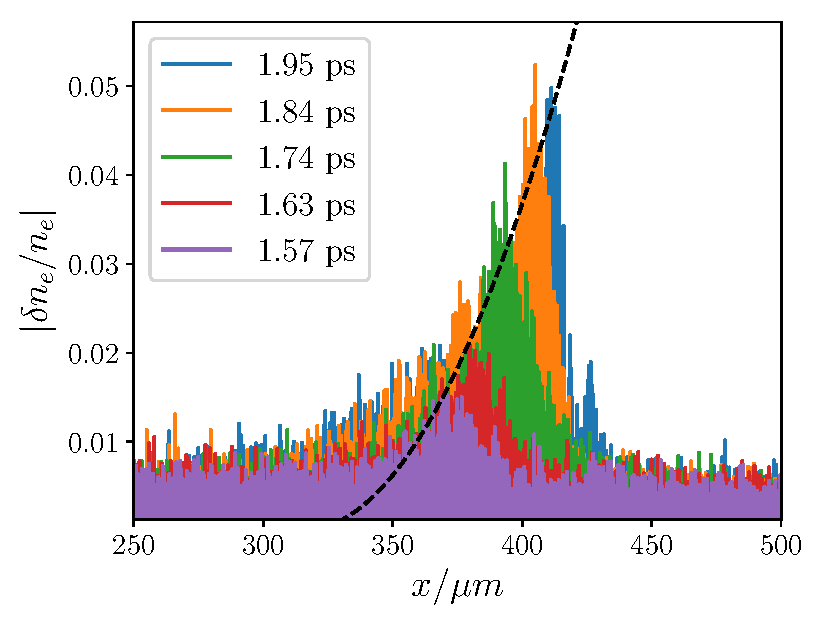
\includegraphics[width=0.8\columnwidth]{Chapters/C2_Theory/AR_diagnostic.pdf}
    \caption{Example of autoresonant growth in an EPOCH simulation with parameters: $n_{min} = 0.06 n_{\text{crit}}$; $n_{max} = 0.17 n_{\text{crit}}$; $T_e = 4.5\si{keV}$; $\text{nPPC}=10,000$; $I_0 = 2 \times 10^{15}\si{\watt / \centi\metre^2}$. Black dashed line comes from Chapman \textit{et al.} \citep{Chapman2012} formula.}
    \label{fig:AR_diagnostic}
\end{figure}{}

%\bibliographystyle{plainnat}
%\bibliography{Chapters/C2_Theory/Theory}
